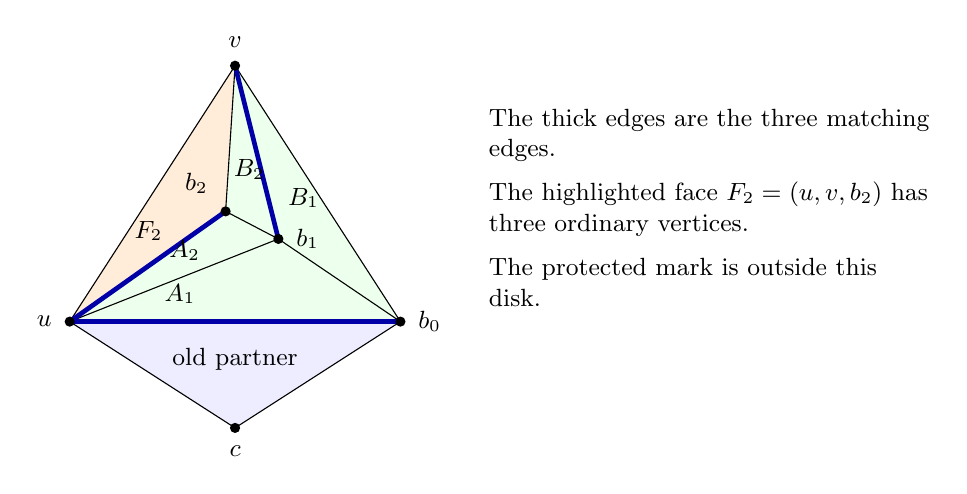
\begin{tikzpicture}[x=1cm,y=1cm,font=\small,
  line cap=round,line join=round,
  vertex/.style={circle,fill=black,inner sep=1.3pt}]
\coordinate (u) at (-2.1,0);
\coordinate (v) at (0,3.25);
\coordinate (b0) at (2.1,0);
\coordinate (b1) at (.55,1.05);
\coordinate (b2) at (-.12,1.40);
\coordinate (c) at (0,-1.35);
\fill[blue!7] (u)--(b0)--(c)--cycle;
\fill[green!7] (u)--(v)--(b0)--cycle;
\fill[orange!15] (u)--(v)--(b2)--cycle;
\draw (u)--(v)--(b0)--cycle;
\draw (u)--(b1)--(v) (b0)--(b1);
\draw (u)--(b2)--(v) (b1)--(b2);
\draw (u)--(c)--(b0);
\draw[line width=1.7pt,blue!65!black] (u)--(b0);
\draw[line width=1.7pt,blue!65!black] (v)--(b1);
\draw[line width=1.7pt,blue!65!black] (u)--(b2);
\foreach \p/\lab/\where in {u/u/left,v/v/above,b0/b_0/right,b1/b_1/right,b2/b_2/above left,c/c/below}{
  \node[vertex] at (\p) {}; \node[\where=3pt] at (\p) {$\lab$};
}
\node at (-1.1,1.15) {$F_2$};
\node at (-.70,.35) {$A_1$};
\node at (-.64,.90) {$A_2$};
\node at (.87,1.57) {$B_1$};
\node at (.18,1.93) {$B_2$};
\node at (0,-.48) {old partner};
\node[align=left,text width=5.6cm,anchor=west] at (3.1,1.45)
  {The thick edges are the three matching edges.\\[5pt]
   The highlighted face $F_2=(u,v,b_2)$ has three ordinary vertices.\\[5pt]
   The protected mark is outside this disk.};
\end{tikzpicture}
